\setlength{\parindent}{4ex}
\setlength{\parskip}{1ex}

\section{Formal Analysis using Alloy}

\subsection{Source code}
		\lstinputlisting[language=alloy]{alloy/SafeStreets.als}

\clearpage
\subsection{Generated Worlds}

\begin{figure}[h!]
	\centering
	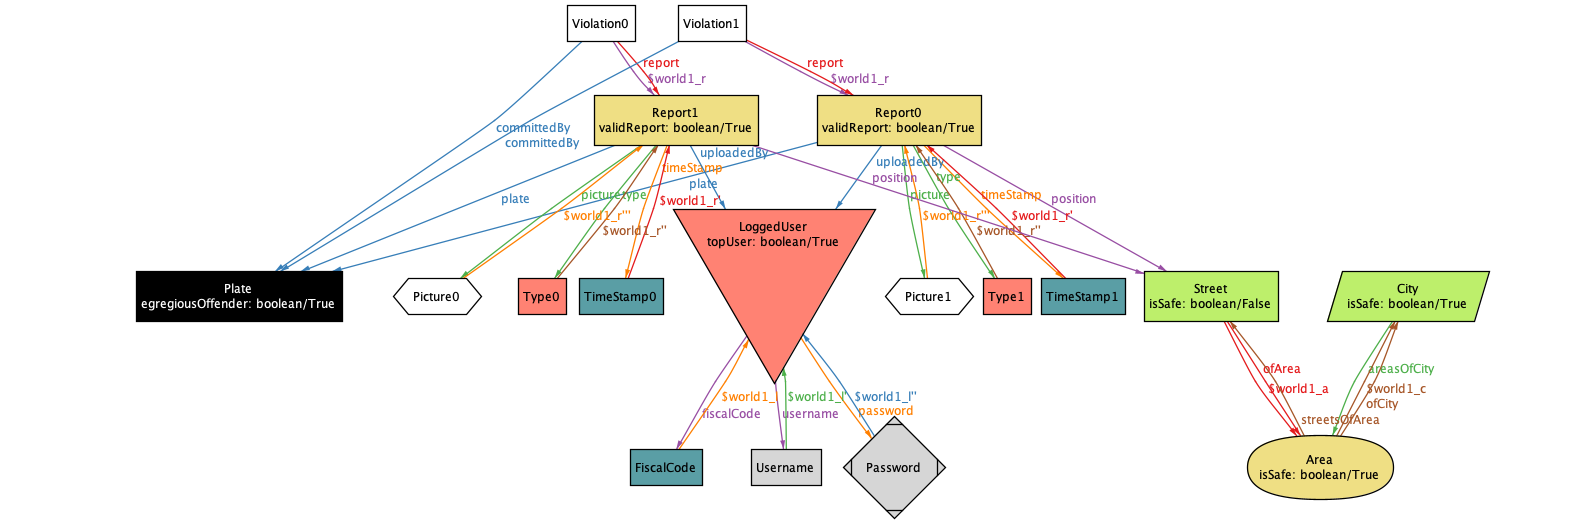
\includegraphics [height=170pt,angle=-90]{alloy/world1.png}
	\caption{
		\label{fig:World1} 
		World 1
	}
\end{figure}

\begin{figure}[h!]
	\centering
	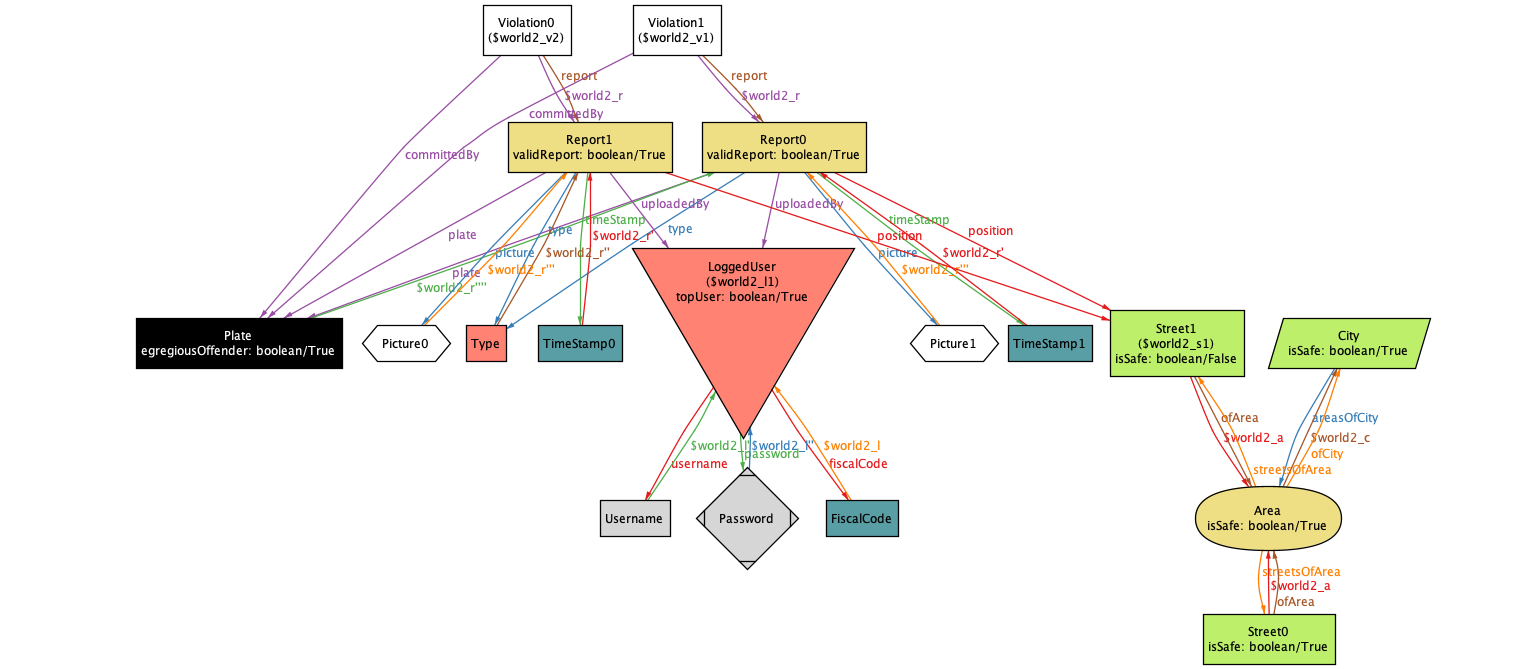
\includegraphics [height=230pt,angle=-90]{alloy/world2.png}
	\caption{
		\label{fig:World2} 
		World 2
	}
\end{figure}

\begin{figure}[h!]
	\centering
	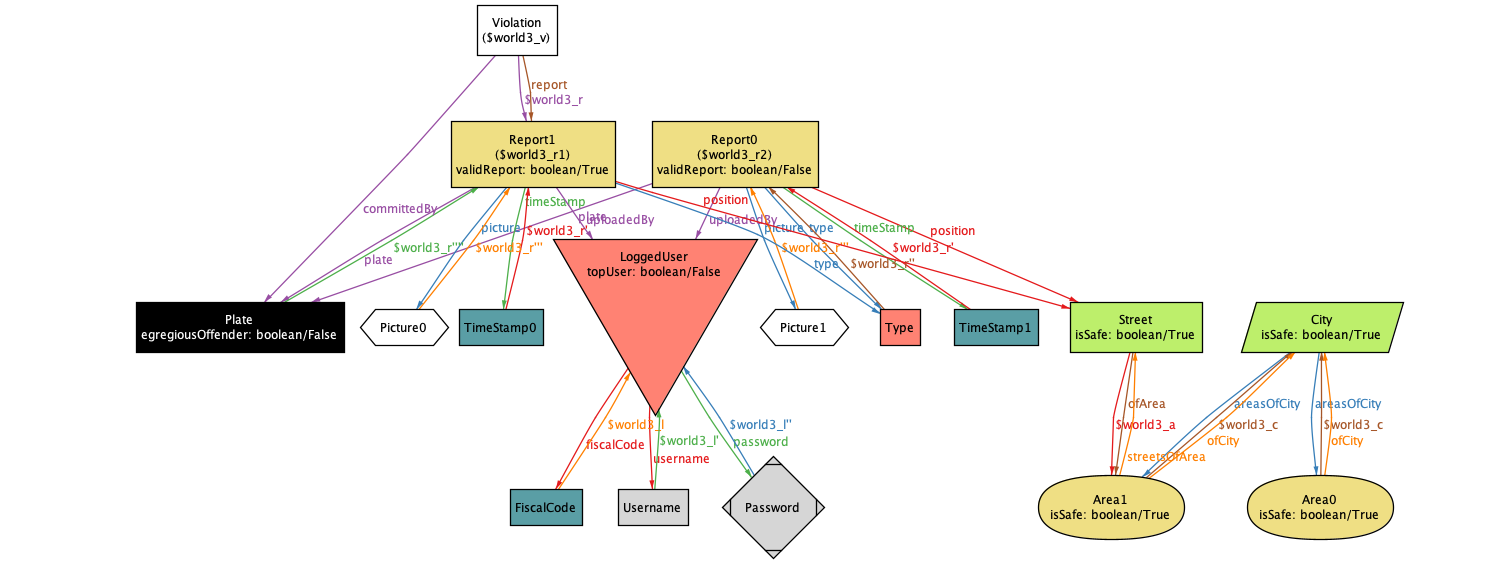
\includegraphics [height=200pt,angle=-90]{alloy/world3.png}
	\caption{
		\label{fig:World3} 
		World 3
	}
\end{figure}

\begin{figure}[h!]
	\centering
	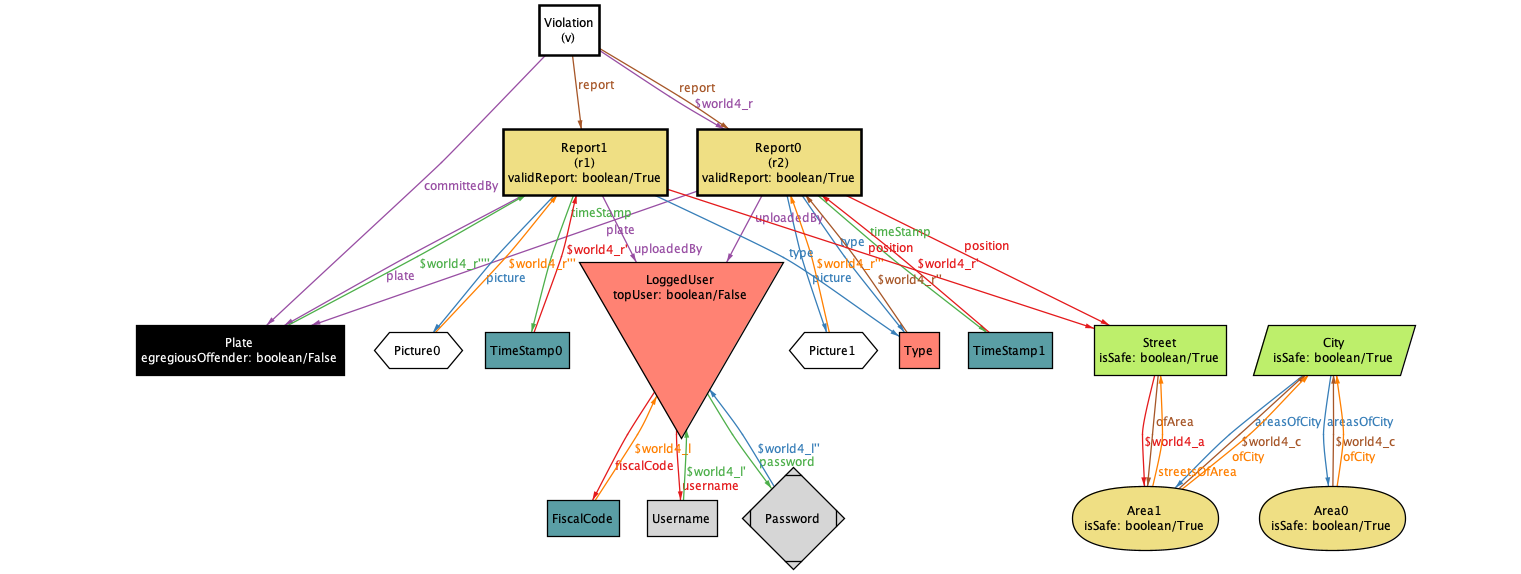
\includegraphics [height=200pt,angle=-90]{alloy/world4.png}
	\caption{
		\label{fig:World4} 
		World 4
	}
\end{figure}

\begin{figure}[h!]
	\centering
	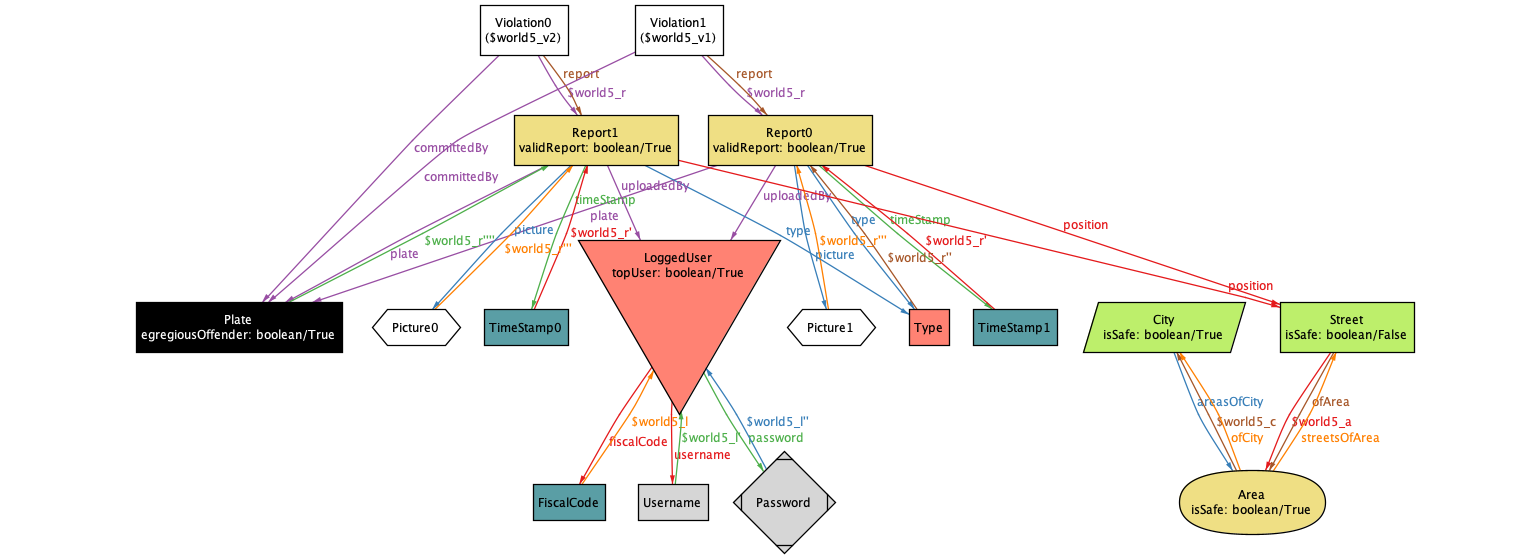
\includegraphics [height=200pt,angle=-90]{alloy/world5.png}
	\caption{
		\label{fig:World5} 
		World 5
	}
\end{figure}

\clearpage

\paragraph{Notes to read the generated worlds}
	\begin{itemize}
		\item The generated \hyperref[fig:World1]{World 1} represents a possible situation in which a LoggedUser acquired the \emph{Top User} label, thanks to its high number of valid submissions.
		
		\item The generated \hyperref[fig:World2]{World 2} represents a possible situation in which Street1 acquired the \emph{Unsafe} label, due to its high number of violations. Street0 is considered \emph{Safe} since no violations occurred in that street.
		
		\item The generated \hyperref[fig:World3]{World 3} represents a possible situation in which Report0 didn't acquire the \emph{Valid Report} label, so it wasn't converted to a Violation.
		
		\item The generated \hyperref[fig:World4]{World 4} represents a possible situation in which two different reports (Report0 and Report1) described the same violation, so they are both connected to the same Violation instance.
		
		\item The generated \hyperref[fig:World5]{World 5} represents a possible situation in which the Plate acquired the \emph{Egregious Offender} label, since it committed two different violations (Violation0 and Violation1).
	\end{itemize}